\documentclass[11pt]{article}

\usepackage[margin=1in]{geometry}
\usepackage{amsmath,amssymb,amsthm,mathtools}
\usepackage{enumitem}
\usepackage{hyperref}
\usepackage{xcolor}
\usepackage{graphicx}
\usepackage{booktabs}
\usepackage{microtype}
\usepackage{titlesec}

\hypersetup{
    colorlinks=true,
    linkcolor=blue,
    urlcolor=blue,
    citecolor=blue
}

\setlength{\parskip}{0.65em}
\setlength{\parindent}{0pt}
\setlist[itemize]{topsep=0.25em,itemsep=0.15em}

\titleformat{\section}{\Large\bfseries}{\thesection.}{0.5em}{}
\titleformat{\subsection}{\large\bfseries}{\thesubsection.}{0.5em}{}

\newtheoremstyle{plainbreak}
{0.8em}{0.8em}{\itshape}{} {\bfseries}{.}{0.5em}{}
\theoremstyle{plainbreak}
\newtheorem{proposition}{Proposition}
\newtheorem{lemma}{Lemma}

\newenvironment{proofblock}[1]{%
    \vspace{0.5em}\hrule\vspace{0.7em}%
    {\bfseries Guided proof block: #1}\par\vspace{0.2em}%
}{%
    \vspace{0.5em}\hrule\vspace{0.7em}%
}

\newenvironment{takeaway}{%
    \vspace{0.4em}\noindent\textbf{Payoff.}\ }{\par\vspace{0.4em}}

\title{A Textbook-Style Explanation of the IRFR One-Factor Model\\
\large Admissible Humped Yield and Volatility Structures with Guided Proof Blocks}
\author{Draft companion note}
\date{}

\begin{document}
\maketitle

\begin{abstract}
This note gives a pedagogical explanation of the instantaneous rolling forward rate (IRFR) framework. The aim is to make the core mechanism transparent: a one-factor rolling-rate model can admit humped yield and volatility term structures without adding extra stochastic factors. The additional shape comes from two deterministic maturity loadings that arise when the maturity-decay scale is separated from the temporal drift-diffusion scale.

The distinction between equilibrium and admissibility is important. The maturity-indexed equilibrium benchmark has a monotone instantaneous volatility profile. Humped volatility is not claimed as a stationary-equilibrium object. Instead, it appears along the non-stationary rolling-maturity branch when the two maturity scales differ. The Kolmogorov Forward Equation nevertheless yields a full maturity-indexed shifted inverse-gamma equilibrium density; all finite moments admitted by that density inherit the equilibrium structure. The exposition follows the main results of the formal paper, but includes guided proof blocks, shape conditions, and stylised numerical examples.
\end{abstract}

\tableofcontents
\newpage

\section{The modelling problem}

Interest-rate models often face a basic tension.

On the one hand, one-factor models are attractive because they are simple, tractable, and easy to interpret. A single Brownian shock drives the whole term structure, so the covariance structure is transparent.

On the other hand, observed yield curves and volatility term structures are often not monotone. In particular, interest-rate volatility is frequently highest at an intermediate maturity rather than at the very short end or the very long end. This is known as a \emph{humped volatility term structure}.

In many standard modelling approaches, a one-factor model struggles to produce this shape naturally. To obtain a volatility hump, one often adds more stochastic factors, imposes a maturity-dependent volatility function, or introduces additional calibration flexibility.

The key question of the IRFR framework is:
\begin{quote}
Can a one-factor model generate humped yield and volatility term structures without adding extra stochastic factors?
\end{quote}

The answer developed in the paper is yes, with an important qualification. The stationary equilibrium benchmark remains monotone. The hump is an admissible off-equilibrium or transitional shape within the rolling-maturity family. The mechanism is not an extra source of randomness. It is the interaction of two deterministic maturity loadings that arise from the rolling structure of the rate being modelled.

\section{The primitive object: the instantaneous rolling forward rate}

The model does not begin with the conventional continuously compounded yield. Instead, it begins with an \emph{instantaneous rolling forward rate}, abbreviated IRFR.

Write this rate as
\[
x_{t,T},
\]
where \(t\) is the current calendar time, \(T\) is the maturity date, and \(T-t\) is the remaining maturity.

The IRFR is the instantaneous forward-type rate associated with a contract maturing at \(T\). As time passes, the same maturity date \(T\) comes closer. Thus the rate naturally \emph{rolls down the maturity curve}.

This rolling feature is central. The model is not treating each maturity as an unrelated point on a static curve. Instead, it treats the forward rate as an object whose local dynamics depend on both its current state and its remaining maturity.

It is useful to define
\[
\tau := T-t.
\]
Then \(\tau\) is the remaining maturity.

The central modelling idea is that the local behaviour of the IRFR should depend on \(x\) and \(\tau\), not separately on \(t\) and \(T\). In other words, two positions with the same rate level and the same remaining maturity should have the same local dynamics, even if they are observed on different calendar dates.

This is the principle of \emph{rolling-maturity invariance}.

\section{Rolling-maturity invariance}

Rolling-maturity invariance says that the local drift and diffusion of the IRFR depend on time only through remaining maturity:
\[
\mu(x,t,T)=\mu(x,T-t),
\]
and
\[
\sigma(x,t,T)=\sigma(x,T-t).
\]

This is a structural consistency condition. Without it, two exposures with the same state and the same remaining maturity could have different instantaneous laws merely because they occur on different calendar dates. That would make the model dependent on the implementation date rather than on the economic exposure.

The point is not that every market must literally satisfy this condition. Rather, the point is that if no additional compensating terms are introduced elsewhere, then the rolling-rate dynamics should be invariant under a simultaneous shift of calendar time and maturity date.

This invariance is one of the ingredients that allows the model to produce a coherent term-structure dynamics.

\section{Affine drift and affine diffusion}

The IRFR density is assumed to satisfy a Kolmogorov Forward Equation. Under the model's affine-closure condition, the drift and diffusion loadings become affine functions of the state variable.

In the paper's notation, one writes the KFE using a drift-diffusion pair \(f\) and \(g\), where \(f\) is the negative of the usual SDE drift and \(g^2\) is half the instantaneous variance coefficient:
\[
f=-\mu, \qquad g^2=\frac{1}{2}\sigma^2.
\]

The KFE becomes
\[
\frac{\partial \phi}{\partial t}
=
\frac{\partial^2}{\partial x^2}(g^2\phi)
+
\frac{\partial}{\partial x}(f\phi).
\]

The affine forms are
\[
f(x,t,T)=a_1(\tau)x+b_1(\tau),
\]
and
\[
g(x,t,T)=a(\tau)x+b(\tau),
\]
where \(\tau=T-t\).

Thus the local dynamics are simple in the state variable: drift is affine, and the diffusion loading is affine. Since the instantaneous variance is proportional to \(g^2\), the variance is quadratic in the state. This places the model in a Pearson-type diffusion family.

This matters because it gives tractability while preserving enough structure to generate nontrivial term-structure shapes.

\begin{proofblock}{why affine forms follow from the KFE}
The starting point is the KFE in \(f,g\) form:
\[
\frac{\partial \phi}{\partial t}
=
\frac{\partial^2}{\partial x^2}(g^2\phi)
+
\frac{\partial}{\partial x}(f\phi).
\]
Expanding the derivatives gives
\[
\frac{\partial \phi}{\partial t}
=
g^2\phi_{xx}
+
\bigl(2(g^2)_x+f\bigr)\phi_x
+
\bigl((g^2)_{xx}+f_x\bigr)\phi.
\]

Rolling-maturity invariance lets us write
\[
f(x,t,T)=F(x,\tau), \qquad g(x,t,T)=G(x,\tau).
\]

The affine-closure hypothesis then imposes two restrictions. First, the diffusion loading has state-independent slope:
\[
\partial_{xx}G(x,\tau)=0.
\]
Therefore \(G\) must be affine in \(x\):
\[
G(x,\tau)=a(\tau)x+b(\tau).
\]

Second, the net probability-flux coefficient is affine in \(x\):
\[
\partial_x(G^2)+F=A(\tau)x+B(\tau).
\]
Because \(G\) is affine, \(\partial_x(G^2)\) is affine. Therefore \(F\) must also be affine:
\[
F(x,\tau)=a_1(\tau)x+b_1(\tau).
\]

Returning to \(f,g\) notation gives
\[
f(x,t,T)=a_1(\tau)x+b_1(\tau),
\qquad
 g(x,t,T)=a(\tau)x+b(\tau).
\]

\begin{takeaway}
The affine drift and affine diffusion loading are not merely convenient guesses. They are the closed form produced by rolling-maturity invariance plus the affine-closure condition applied to the KFE.
\end{takeaway}
\end{proofblock}

\section{The equilibrium curve}

The model introduces an equilibrium maturity curve
\[
x_{e,\tau}.
\]

This is not a calendar-time stationary limit. It is a maturity-indexed equilibrium object: for each remaining maturity \(\tau\), it describes the equilibrium level associated with that maturity.

The equilibrium curve is assumed to converge to a long-maturity regime level:
\[
\lim_{\tau\to\infty}x_{e,\tau}=x_\infty.
\]

A natural exponential form is used:
\[
x_{e,\tau}=x_\infty+A e^{-\lambda^2\tau}.
\]

Here \(x_\infty\) is the long-maturity level, \(A\) determines the short-end displacement, and \(\lambda^2\) is the maturity-decay scale.

A key point of the revised framework is that \(\lambda^2\) need not equal the temporal drift-diffusion scale \(a^2\). This separation is the main source of the model's richer behaviour.

\section{The scale ratio \texorpdfstring{\(r\)}{r}}

The model identifies the drift scale with the squared diffusion loading:
\[
a_1=a^2.
\]

But it does not force the maturity-decay scale to equal \(a^2\). Instead, it defines
\[
r:=\frac{\lambda^2}{a^2}>0.
\]
Equivalently,
\[
\lambda^2=ra^2.
\]

The parameter \(r\) measures the relative speed of maturity decay compared with temporal drift-diffusion propagation.

This is the crucial parameter:
\begin{itemize}
    \item If \(r=1\), the maturity-decay scale and temporal scale coincide.
    \item If \(r\neq 1\), the model has two distinct maturity decay speeds.
\end{itemize}

The earlier one-scale model is therefore the special branch \(r=1\). The general model is the full \(r>0\) family.

\section{Positivity and the short end}

The IRFR is required to remain positive at zero maturity. This is imposed through the condition that the diffusion loading vanishes at the zero-maturity boundary.

This condition determines the amplitude \(A\) in the equilibrium curve. Starting from
\[
x_{e,\tau}=x_\infty+A e^{-ra^2\tau},
\]
positivity at the short end gives
\[
A=-\frac{x_\infty}{1+r}.
\]
Therefore the equilibrium curve becomes
\[
x_{e,\tau}
=
x_\infty\left(1-\frac{1}{1+r}e^{-ra^2\tau}\right).
\]
At zero maturity, this gives
\[
x_{e,0}=\frac{r}{1+r}x_\infty.
\]

This is important. The familiar one-half result
\[
x_{e,0}=\frac{1}{2}x_\infty
\]
is not general. It occurs only when \(r=1\). Thus the short end is controlled by the scale ratio \(r\).

\begin{proofblock}{how positivity fixes the amplitude \(A\)}
Before imposing the boundary condition, the interim diffusion loading implied by the exponential equilibrium curve has the form
\[
g(x,t,T)
=
a x_{t,T}-a x_\infty-
\left(a+\frac{\lambda^2}{a}\right)A e^{-\lambda^2(T-t)}.
\]
At zero maturity, \(T=t\), so \(e^{-\lambda^2(T-t)}=1\). The short-end boundary is \(x_{t,t}=0\). Positivity is imposed by requiring the diffusion loading to vanish at this boundary:
\[
g(0,t,t)=0.
\]
Therefore
\[
0=-a x_\infty-
\left(a+\frac{\lambda^2}{a}\right)A.
\]
Using \(\lambda^2=ra^2\), we have
\[
a+\frac{\lambda^2}{a}=a+ra=a(1+r).
\]
Thus
\[
0=-a x_\infty-a(1+r)A.
\]
Dividing by \(-a\) gives
\[
x_\infty+(1+r)A=0,
\]
so
\[
A=-\frac{x_\infty}{1+r}.
\]

\begin{takeaway}
The amplitude is not freely calibrated in this structural version of the model. It is fixed by the requirement that the short-end diffusion vanish at the zero boundary.
\end{takeaway}
\end{proofblock}

\section{The general forward curve}

The model gives the following forward-curve representation:
\[
x_{t,T}
=
x_\infty
-
\frac{x_\infty}{1+r}e^{-ra^2(T-t)}
+
\left(x_{t,t}-\frac{r}{1+r}x_\infty\right)e^{-a^2(T-t)}.
\]

Using \(\tau=T-t\), this becomes
\[
x_t(\tau)
=
x_\infty
-
\frac{x_\infty}{1+r}e^{-ra^2\tau}
+
\left(x_{t,t}-\frac{r}{1+r}x_\infty\right)e^{-a^2\tau}.
\]

This formula is the heart of the model. It contains two maturity loadings:
\[
e^{-a^2\tau}
\]
and
\[
e^{-ra^2\tau}.
\]

When \(r=1\), these are the same loading, so the curve collapses to a single exponential form.

When \(r\neq 1\), the two loadings decay at different speeds. Their interaction allows the curve to be monotone, inverted, or humped, even though the stochastic model has only one Brownian driver.

This is the first major modelling payoff.

\section{Why a one-factor model can generate a hump}

A standard one-factor model often produces term structures whose shapes are tightly constrained by a single maturity loading.

Here, the model remains one-factor in its randomness, but not one-loading in its maturity geometry.

The forward curve has the schematic form
\[
x_t(\tau)=x_\infty+C_1 e^{-a^2\tau}+C_2 e^{-ra^2\tau}.
\]
The constants \(C_1\) and \(C_2\) depend on the short-end rate, \(x_\infty\), and \(r\).

A sum of two exponentials can have an interior turning point when the two terms have different signs or sufficiently different decay rates. Therefore the curve can rise at first and then fall, or fall at first and then rise.

The stochastic dimension has not increased. There is still one Brownian shock. The additional shape comes from deterministic maturity structure.

That is the main conceptual insight.

\section{The volatility term structure}

The same mechanism appears in the local variance-rate.

For the IRFR, the instantaneous variance-rate has the form
\[
\frac{\partial}{\partial t}\operatorname{Var}(x_{t,T})
=
2a^2
\left[
\left(
x_{t_0,t_0}
-
\frac{r}{1+r}x_\infty
\right)
e^{-a^2(T+t-2t_0)}
+
\frac{r}{1+r}x_\infty e^{-ra^2(T-t)}
\right]^2.
\]

For fixed calendar time \(t\), this is again a two-loading maturity function. In schematic form,
\[
v_x(\tau)
=
2a^2\left(Ae^{-a^2\tau}+Be^{-ra^2\tau}\right)^2.
\]

Because \(r\neq 1\) gives two distinct maturity scales, the local variance can be highest at an intermediate maturity. This is the humped-volatility result.

The important point is that the hump is not caused by a second Brownian motion. It is caused by the interaction of two deterministic maturity loadings inside a one-factor covariance structure.

\begin{proofblock}{when the volatility hump appears}
For fixed \(t\), write the local variance-rate in the simplified form
\[
v_x(\tau)=2a^2H(\tau)^2,
\qquad
H(\tau)=A e^{-a^2\tau}+B e^{-ra^2\tau}.
\]
The derivative is
\[
v_x'(\tau)=4a^2H(\tau)H'(\tau),
\]
where
\[
H'(\tau)=-a^2A e^{-a^2\tau}-ra^2B e^{-ra^2\tau}.
\]
An interior critical point of the variance-rate can therefore occur either when \(H(\tau)=0\), giving a zero of variance, or when
\[
H'(\tau)=0.
\]
The nonzero turning-point condition is
\[
A e^{-a^2\tau}+rB e^{-ra^2\tau}=0.
\]
Equivalently,
\[
e^{-(1-r)a^2\tau}=-\frac{rB}{A}.
\]
Thus an interior nonzero turning point exists when \(-rB/A>0\) and the resulting maturity
\[
\tau^*=-\frac{1}{(1-r)a^2}\log\left(-\frac{rB}{A}\right)
\]
is positive.

At such a point, \(H'(\tau^*)=0\). The second derivative is
\[
v_x''(\tau^*)=4a^2H(\tau^*)H''(\tau^*),
\]
where
\[
H''(\tau)=a^4 A e^{-a^2\tau}+r^2a^4B e^{-ra^2\tau}.
\]
Using the critical-point relation, this can be checked directly for a strict local maximum in the relevant parameter region. In particular, when the two exponential components have opposite signs and different decay rates, the magnitude \(|H(\tau)|\) can be largest away from the short end, producing a volatility hump.

The covariance-rate kernel remains one-factor. If
\[
\frac{\partial}{\partial t}\operatorname{Var}(x_{t,S})=2a^2H(S)^2,
\]
then the one-Brownian-driver structure gives
\[
\frac{\partial}{\partial t}\operatorname{Cov}(x_{t,S_1},x_{t,S_2})
=2a^2H(S_1)H(S_2).
\]
This is rank one.

\begin{takeaway}
The hump comes from the deterministic maturity profile \(H(\tau)\), not from a second stochastic factor. The model is one-factor in randomness but two-loading in maturity.
\end{takeaway}
\end{proofblock}


\section{Stationary equilibrium versus admissible humped volatility}

It is important not to overstate what the humped-volatility result says.

The model does not claim that the stationary or maturity-indexed equilibrium volatility curve is humped. In the equilibrium benchmark, the instantaneous volatility loading is monotone in maturity and declines away from the short end. This is consistent with the usual intuition that single-factor stationary term-structure models have difficulty producing stationary humped volatility profiles.

The contribution is different. The model shows that humped volatility is admissible in a structurally consistent one-factor rolling-rate framework once the maturity-decay scale and temporal drift-diffusion scale are allowed to differ. The hump belongs to the non-stationary rolling-maturity branch, not to the stationary equilibrium benchmark.

This distinction matters because it prevents a false contradiction with standard one-factor restrictions. The model does not evade those restrictions by imposing an exogenous humped volatility function. Nor does it introduce a second Brownian factor. Instead, it shows that the admissible one-factor family contains non-stationary term structures whose local volatility profile may be humped.

Axiom 3 imposes equilibrium transport only on the first two moments. It does not, by itself, assume a full stationary distribution for all higher-order moments. However, the KFE solution later provides a full maturity-indexed shifted inverse-gamma equilibrium density. Hence all finite moments admitted by that density inherit the equilibrium structure.

\begin{takeaway}
Stationary equilibrium is monotone. Humped volatility is an admissible non-stationary rolling-maturity shape. This is the key conceptual distinction.
\end{takeaway}

\section{One factor, but two loadings}

The phrase ``one-factor'' refers to the number of stochastic drivers. In this model, there is one Brownian motion.

However, the maturity profile can involve more than one deterministic loading. This distinction is crucial.

A model can be one-factor in randomness while still having a richer deterministic maturity geometry.

In the IRFR framework:
\begin{itemize}
    \item the randomness is one-dimensional;
    \item the covariance kernel remains rank one;
    \item the maturity profile contains two exponential loadings when \(r\neq 1\).
\end{itemize}

Thus the model can generate humped volatility without abandoning one-factor tractability.

This is the main reason the general \(r\)-branch is economically important.


\section{Admissible yield-curve shapes}

The same two-loading mechanism that generates humped volatility can also generate a richer set of deterministic yield-curve shapes. The equilibrium benchmark is monotone, but admissible non-stationary curves can be upward-sloping, downward-sloping, humped, or locally dipped.

A notational caution is important. The quantity \(x_{t_0,t_0}\) is not a structural parameter of the model. It is the short-end boundary value observed at the reconstruction date \(t_0\). Once that boundary value is fixed by the observed curve, it imposes a level restriction on the admissible maturity profile. In particular, in the two-loading representation below the constants \(A\) and \(B\) cannot both be chosen independently after \(x_{t_0,t_0}\) has been observed; they must satisfy \(A+B=x_{t_0,t_0}-x_\infty\). The stylised graphs therefore vary the admissible loading split to illustrate possible shapes. They do not introduce \(x_{t_0,t_0}\) as a freely calibrated parameter alongside \(a^2\), \(r\), or \(x_\infty\).

\begin{proofblock}{conditions for humped yield curves}
A convenient way to see the admissible yield-curve shapes is to write a stylised two-loading initial rolling forward curve as
\begin{equation*}
    x(t_0,t_0+\tau)=x_\infty+A e^{-a^2\tau}+B e^{-ra^2\tau},
\end{equation*}
with
\begin{equation*}
    A+B=\Delta,
    \qquad
    \Delta:=x_{t_0,t_0}-x_\infty.
\end{equation*}
The associated conventional continuously compounded yield is
\begin{equation*}
    y(t_0,t_0+\tau)
    =x_\infty
    +A\frac{1-e^{-a^2\tau}}{a^2\tau}
    +B\frac{1-e^{-ra^2\tau}}{ra^2\tau}.
\end{equation*}

The short-end slope follows from
\begin{equation*}
    \frac{1-e^{-k\tau}}{k\tau}=1-\frac{k\tau}{2}+O(\tau^2).
\end{equation*}
Therefore
\begin{equation*}
    \frac{\partial y(t_0,t_0+\tau)}{\partial \tau}\bigg|_{\tau=0}
    =-\frac{a^2}{2}(A+rB)
    =-\frac{a^2}{2}\bigl[\Delta+(r-1)B\bigr].
\end{equation*}
Thus the conventional yield curve initially slopes upward if
\begin{equation*}
    \Delta+(r-1)B<0,
\end{equation*}
and initially slopes downward if
\begin{equation*}
    \Delta+(r-1)B>0.
\end{equation*}

The long-maturity approach is governed by
\begin{equation*}
    y(t_0,t_0+\tau)-x_\infty
    \sim
    \frac{1}{a^2\tau}\left(A+\frac{B}{r}\right),
    \qquad \tau\to\infty.
\end{equation*}
Since
\begin{equation*}
    A+\frac{B}{r}
    =\Delta-\left(1-\frac{1}{r}\right)B,
\end{equation*}
this sign determines whether the conventional yield approaches the long-maturity level from above or below.

A sufficient condition for an initially upward-sloping curve to have an interior hump is therefore
\begin{equation*}
    \Delta+(r-1)B<0
\end{equation*}
together with
\begin{equation*}
    \Delta-\left(1-\frac{1}{r}\right)B>0.
\end{equation*}
The first inequality makes the curve rise away from the short end. The second makes the long end approach the asymptote from above, so the curve must eventually turn down.

For example, condition on an observed short-end boundary value
\begin{equation*}
    x_{t_0,t_0}=2.00\%,
    \qquad x_\infty=3.00\%,
    \qquad a^2=0.25,
    \qquad r=4.
\end{equation*}
Then \(\Delta=-1.00\%\). An admissible loading split is
\begin{equation*}
    B=-2.50\%,
    \qquad A=1.50\%,
\end{equation*}
gives \(A+B=-1.00\%\). The curve rises from a low short rate, moves above the long-maturity level, and then declines back toward \(x_\infty\).

A second admissible hump is possible even when the observed short rate starts above the long-maturity level. For example, condition on
\begin{equation*}
    x_{t_0,t_0}=3.50\%,
    \qquad x_\infty=2.50\%,
    \qquad a^2=0.25,
    \qquad r=4,
\end{equation*}
and choose the admissible split
\begin{equation*}
    B=-2.00\%,
    \qquad A=3.00\%.
\end{equation*}
Then \(A+B=1.00\%\). The short rate already lies above the long-maturity level, but the yield curve can still rise initially before turning down.

The same two-loading structure can generate positive or negative single-turning-point shapes, depending on the relative signs and magnitudes of the maturity loadings. More complex multi-turning-point curves should not be viewed as a feature of the bare structural benchmark; they would naturally point to policy intervention, market segmentation, or another exogenous distortion.

\begin{takeaway}
The scale parameters \(a^2\) and \(r\) set the maturity clocks. The observed short-end value \(x_{t_0,t_0}\) fixes the boundary level at the reconstruction date; it is data, not an additional structural parameter. Conditional on that boundary, the admissible loading split between \(A\) and \(B\) determines whether the reconstructed curve is monotone, humped, or locally dipped.
\end{takeaway}
\end{proofblock}

\begin{figure}[h!]
    \centering
    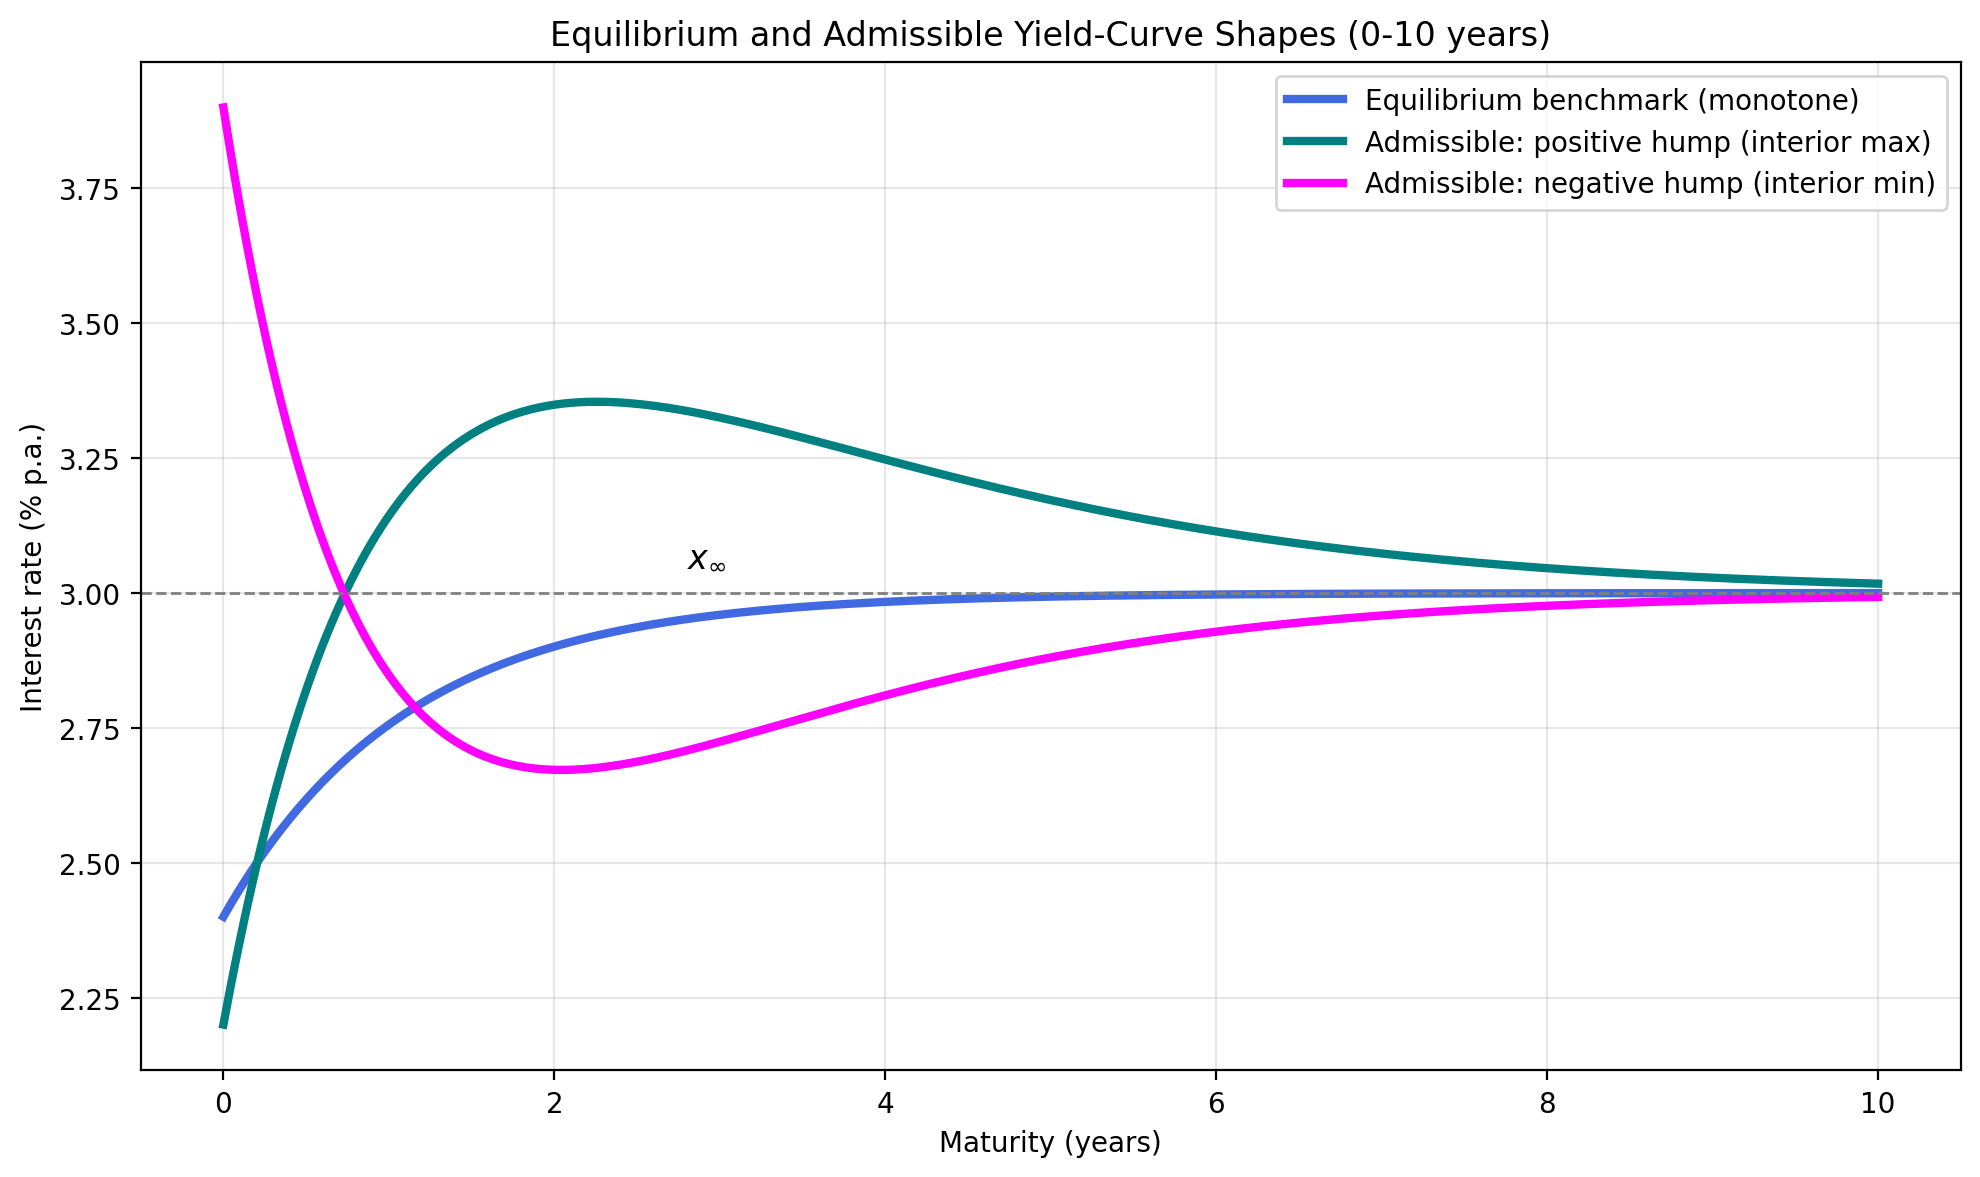
\includegraphics[width=0.90\textwidth]{fig_equilibrium_admissible_yield_shapes.png}
    \caption{Equilibrium and admissible yield-curve shapes over the 0--10 year maturity range. The blue curve shows the monotone equilibrium benchmark converging to the long-maturity level \(x_\infty\). The teal curve illustrates an admissible positive hump with an interior maximum, while the magenta curve illustrates an admissible negative hump with an interior minimum. The two humped curves are stylised off-equilibrium examples and are not stationary-equilibrium volatility claims. The short-end value \(x_{t_0,t_0}\) is the observed boundary value of the reconstructed curve, not a freely chosen structural parameter.}
    \label{fig:admissible-yield-shapes}
\end{figure}

Figure~\ref{fig:admissible-yield-shapes} gives a visual summary of the preceding shape discussion. The equilibrium benchmark is monotone, but admissible non-stationary curves can exhibit either a positive hump or a negative hump depending on the relative signs and magnitudes of the two maturity loadings. The figure is purely illustrative; it is intended to separate the equilibrium benchmark from the broader admissible family of observed or reconstructed curves. In particular, the figure does not introduce \(x_{t_0,t_0}\) as a free graphing parameter or structural parameter. It treats \(x_{t_0,t_0}\) as the short-end boundary condition observed at \(t_0\).

\section{A caution about empirical calibration}

The two-loading structure gives useful flexibility for matching observed curves. However, the bare model should not be interpreted as a complete empirical description of every observed term structure.

In practice, short and intermediate maturities may be affected by central-bank policy, administered rates, quantitative easing, liquidity regulation, collateral scarcity, and other institutional interventions. These forces can create local distortions that are not part of the undisturbed rolling-maturity benchmark.

For empirical testing and practitioner application, the natural extension is therefore to add a policy-intervention or exogenous-distortion component. The present model is best understood as the structurally admissible one-factor benchmark against which such interventions can be measured.

\section{Conventional rates}

The conventional continuously compounded rate over \([t,T]\) is the maturity average of the IRFR:
\[
r_{t,T}=\frac{1}{T-t}\int_t^T x_{t,S}\,dS.
\]

Substituting the general IRFR curve gives
\[
r_{t,T}
=
x_\infty
-
\frac{x_\infty}{1+r}\frac{1-e^{-ra^2(T-t)}}{ra^2(T-t)}
+
\left(x_{t,t}-\frac{r}{1+r}x_\infty\right)
\frac{1-e^{-a^2(T-t)}}{a^2(T-t)}.
\]

So conventional rates inherit the same two-scale structure.

This matters because the model's non-monotone behaviour is not an artifact of using the IRFR as the primitive. Once the IRFR is averaged into a conventional rate, the two maturity scales remain.

The same is true for the local variance-rate of conventional rates. The averaging changes the loading functions, but it does not eliminate the two-scale mechanism.

Thus both forward rates and conventional rates can display humped term structures in a one-factor framework.


\section{Stylised numerical illustration}

The following stylised example shows that an ordinary upward-sloping conventional yield curve can coexist with a humped conventional-rate instantaneous volatility profile. As above, \(x_{t_0,t_0}\) is the observed short-end boundary value for the curve being illustrated. It is not an extra structural parameter added to the model.

Condition on
\begin{equation*}
    x_\infty=4.00\%,
    \qquad x_{t_0,t_0}=0.50\%,
    \qquad a=0.70,
    \qquad a^2=0.49,
    \qquad r=0.30,
    \qquad t=t_0.
\end{equation*}
The conventional yield curve is upward sloping and non-inverted. The front-end yield is approximately \(0.50\%\), the two-year yield is approximately \(1.06\%\), the ten-year yield is approximately \(2.30\%\), and the thirty-year yield is approximately \(3.28\%\).

Under the same parameter set, the conventional-rate instantaneous volatility is non-zero for finite maturity and has an interior maximum near the two-year sector. In this example, the maximum occurs at approximately \(1.96\) years.

\begin{figure}[h!]
    \centering
    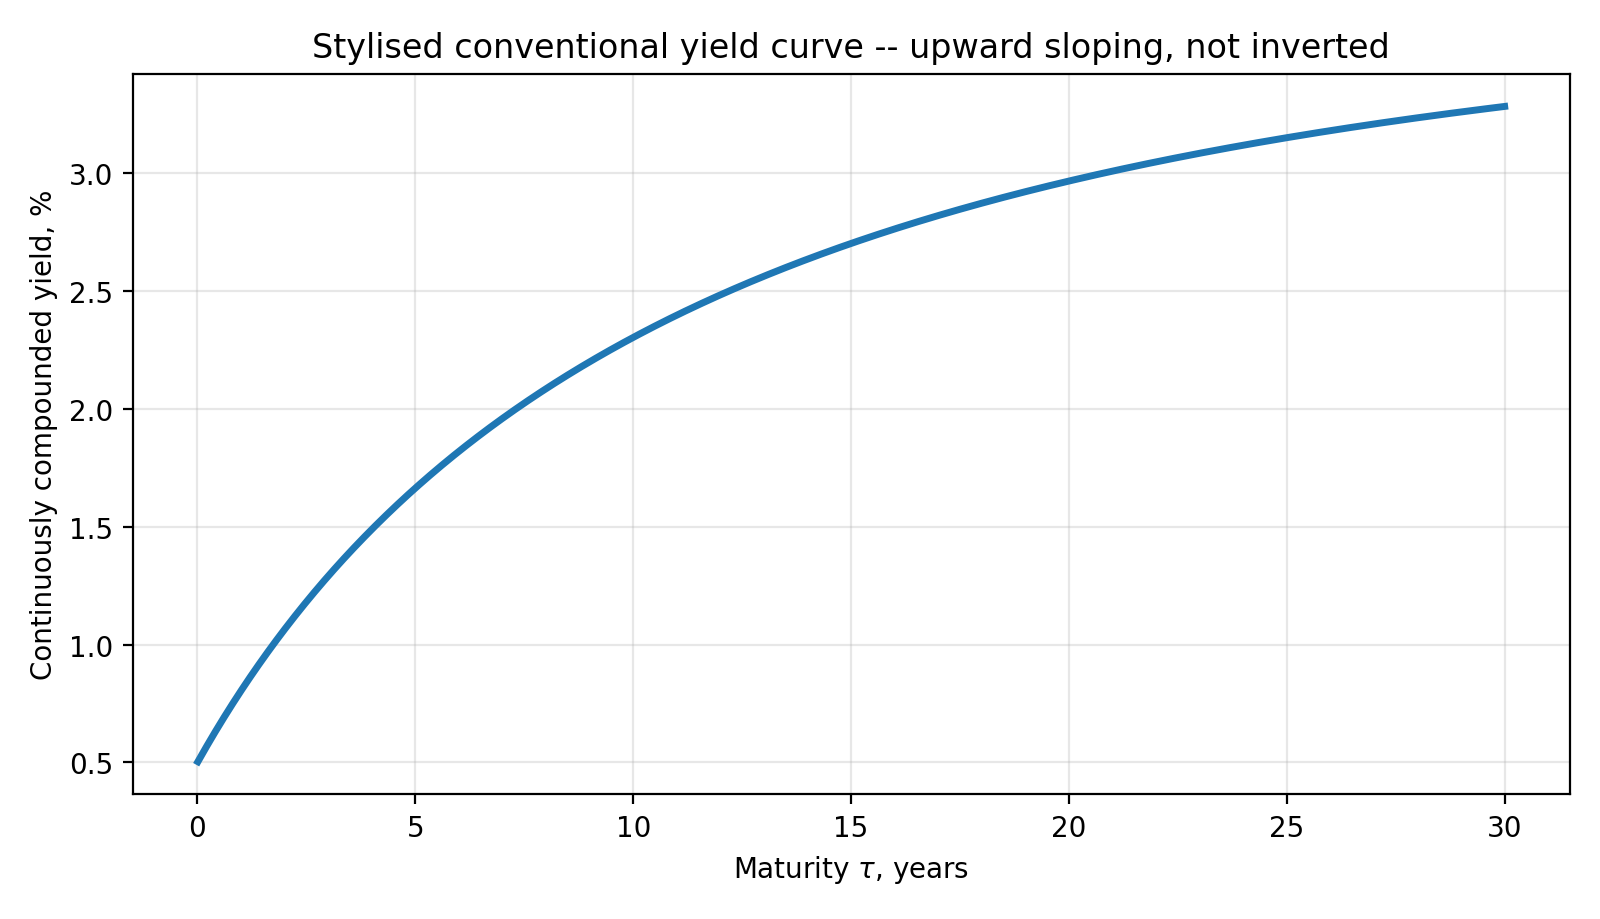
\includegraphics[width=0.82\textwidth]{fig_conventional_yield_curve_first_example.png}
    \caption{Stylised upward-sloping conventional yield curve under the general \(r\)-branch.}
\end{figure}

\begin{figure}[h!]
    \centering
    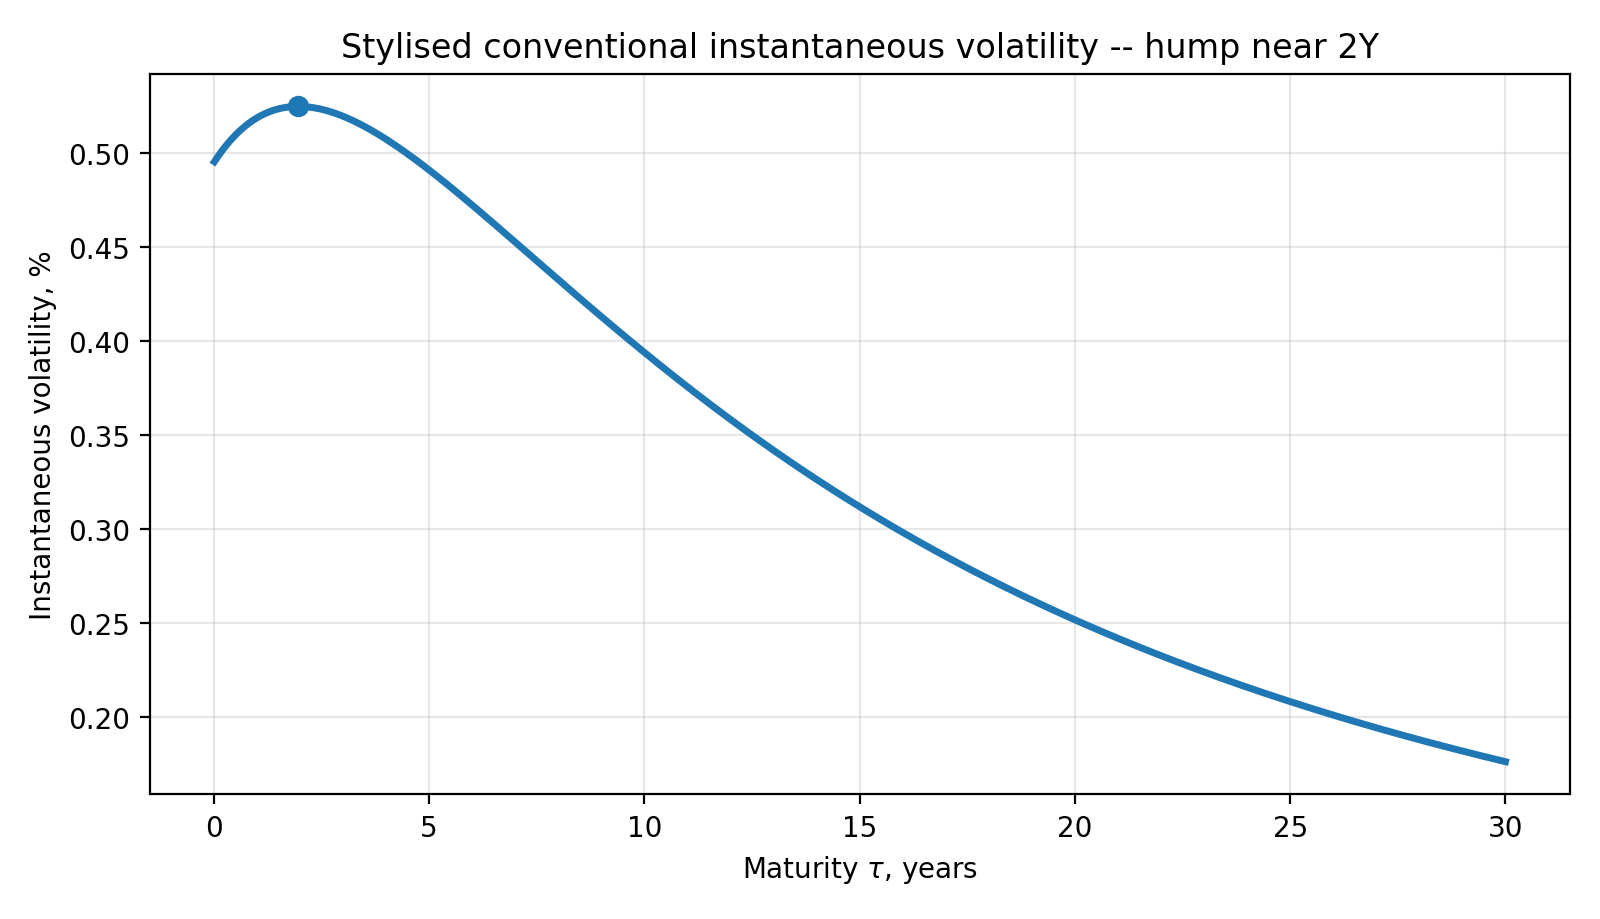
\includegraphics[width=0.82\textwidth]{fig_conventional_vol_hump_first_example.png}
    \caption{Stylised conventional-rate instantaneous volatility under the same parameter set. The volatility is non-zero for finite maturity and has an interior hump close to two years.}
\end{figure}

\begin{takeaway}
The yield curve shape and the volatility shape are different objects. A normal upward-sloping yield curve can coexist with a humped local volatility profile in the same one-factor specification.
\end{takeaway}

\section{Equilibrium density}

The Kolmogorov Forward Equation also yields a maturity-indexed equilibrium density.

In the shifted coordinate
\[
\widetilde{x}^{(r)}_{t,T}
=
x_{t,T}
-
x_\infty\left(1-e^{-ra^2(T-t)}\right),
\]
one obtains
\[
\widetilde{x}^{(r)}_{t,T}
\sim
\operatorname{InvGamma}
\left(
r+2,
rx_\infty e^{-ra^2(T-t)}
\right).
\]

Equivalently, the density is
\[
\phi(\widetilde{x}^{(r)}_{t,T})
=
\frac{
\left(rx_\infty e^{-ra^2(T-t)}\right)^{r+2}
}{
\Gamma(r+2)
\left(\widetilde{x}^{(r)}_{t,T}\right)^{r+3}
}
\exp\left(
-
\frac{rx_\infty e^{-ra^2(T-t)}}{\widetilde{x}^{(r)}_{t,T}}
\right),
\qquad \widetilde{x}^{(r)}_{t,T}>0.
\]

The old order-three density corresponds to \(r=1\), since then the shape parameter is \(r+2=3\).

Thus the KFE does not merely give a single special inverse-gamma law. It gives a family of shifted inverse-gamma laws indexed by the maturity-scale ratio \(r\).

The moment statement should be read with the usual inverse-gamma qualification. If
\[
\widetilde{x}^{(r)}_{t,T}\sim \operatorname{InvGamma}(r+2,\beta),
\]
then the \(n\)-th raw moment exists only for
\[
n<r+2.
\]
Therefore the equilibrium density supplies a full maturity-indexed distributional structure, and all finite moments admitted by that distribution inherit the corresponding equilibrium behaviour.

\subsection{Comparison with gamma and Gaussian benchmarks}

To make the shifted inverse-gamma equilibrium law more intuitive, it is helpful to compare it with two familiar one-factor benchmark distributions: a gamma law, which is representative of positive-state CIR-style specifications, and a Gaussian law, which is representative of Vasicek-style specifications.

The comparison in Figure~\ref{fig:density-comparison} is purely illustrative. The shifted inverse-gamma density is taken to have order three, so that
\[
\widetilde{x}_{t,T}\sim \operatorname{InvGamma}(3,\beta),
\]
and the plotted rate level is the shifted variable
\[
x = c + \widetilde{x}_{t,T},
\]
with lower boundary at \(c=1.00\%\). The scale is chosen as \(\beta=4.00\%\), which implies a mean of \(3.00\%\) and a standard deviation of \(2.00\%\). The gamma and Gaussian benchmark densities are then chosen to have the same mean and variance as the shifted inverse-gamma law.

This common-moment normalization makes the shape comparison more informative. The shifted inverse-gamma law is more strongly right-skewed and more heavy-tailed than the gamma benchmark, while the Gaussian benchmark assigns probability mass to negative rates. The figure therefore clarifies the distinctive distributional implications of the present framework relative to classical one-factor benchmark models.

\begin{figure}[h!]
    \centering
    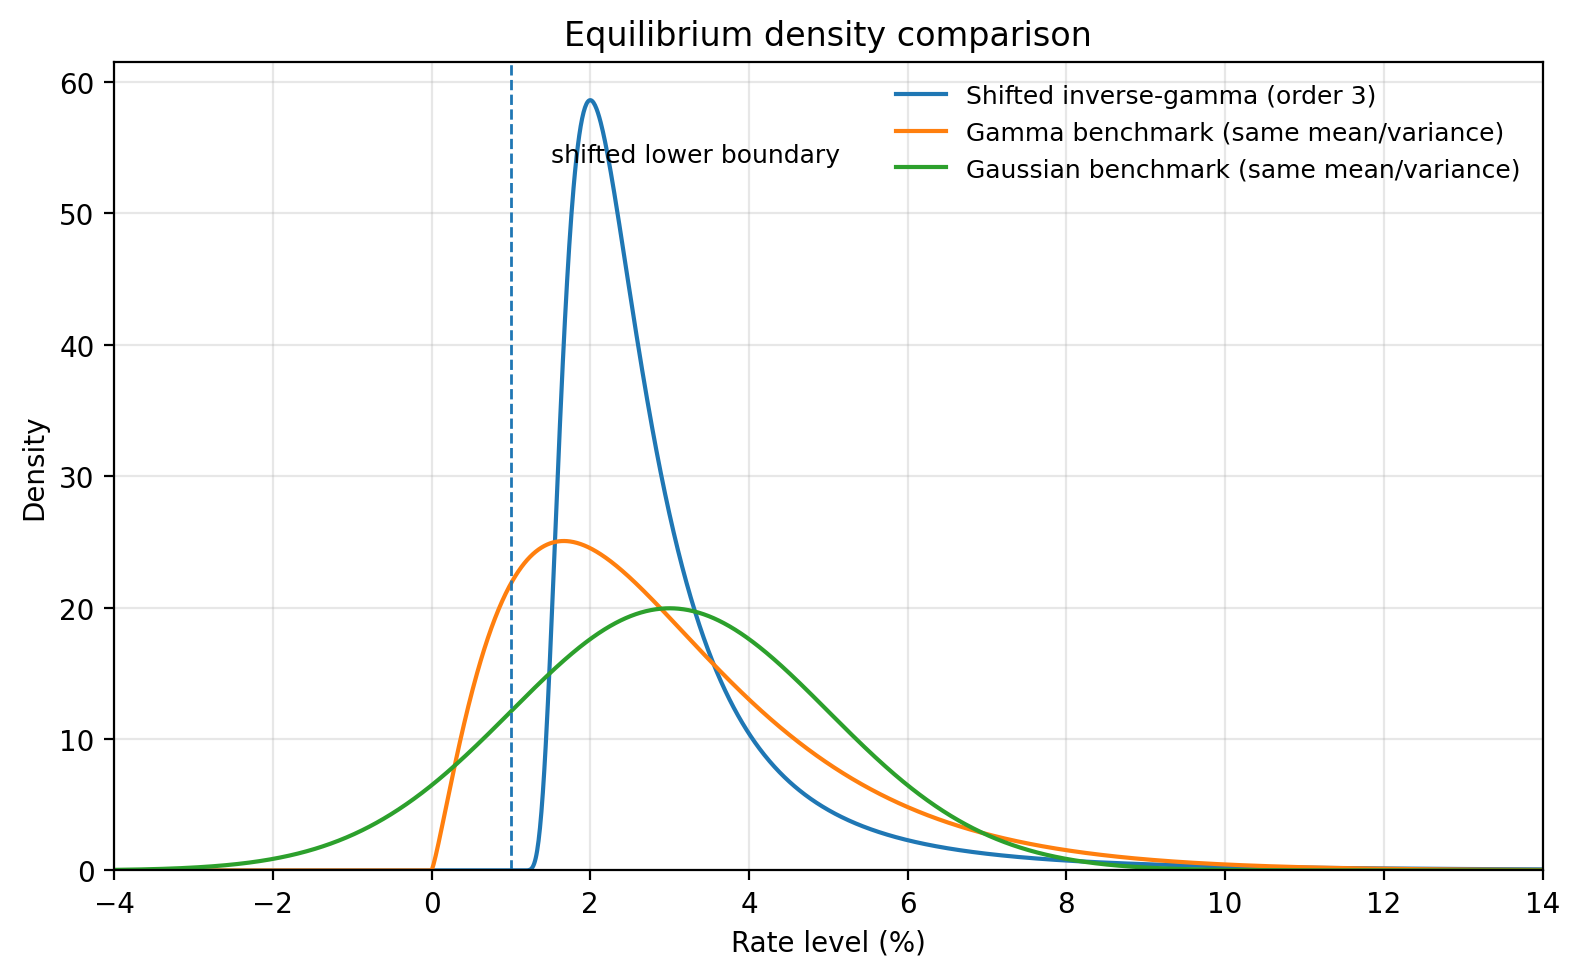
\includegraphics[width=0.86\textwidth]{fig_density_comparison_inversegamma_gamma_gaussian.png}
    \caption{Comparison of equilibrium density shapes. The figure compares a shifted inverse-gamma density of order 3 with gamma and Gaussian benchmark densities calibrated to the same mean and variance. The shifted inverse-gamma law is more strongly right-skewed and more heavy-tailed than the gamma benchmark, while the Gaussian benchmark assigns probability mass to negative values. The dashed vertical line marks the shifted lower boundary.}
    \label{fig:density-comparison}
\end{figure}

\begin{takeaway}
The equilibrium law in the present framework is not merely positive. It has a characteristic shifted, right-skewed, heavy-tailed shape that differs visibly from both CIR-style gamma benchmarks and Vasicek-style Gaussian benchmarks.
\end{takeaway}

\begin{proofblock}{why the inverse-gamma density appears}
The key is to work in the shifted coordinate
\[
\widetilde{x}^{(r)}_{t,T}
=
x_{t,T}-x_\infty\left(1-e^{-ra^2(T-t)}\right),
\]
where the drift and diffusion loadings are proportional to \(\widetilde{x}^{(r)}_{t,T}\).

Introduce the reciprocal variable
\[
z=\frac{1}{\widetilde{x}^{(r)}_{t,T}}.
\]
Near the lower shifted boundary, this reciprocal coordinate is natural because inverse-gamma densities become exponential-polynomial functions of \(z\).

Seek a Frobenius expansion
\[
\phi(z,t,T)=\sum_{i=0}^{\infty}c_i(t)z^{i+m}.
\]
Substitution into the transformed KFE yields a coefficient recurrence. The inverse-gamma branch is the branch for which the recurrence reduces to
\[
\frac{c_i^*}{c_{i-1}^*}=-\frac{r}{i}.
\]
This recurrence sums to an exponential series:
\[
\sum_{i=0}^{\infty}\frac{(-r)^i}{i!}w^i = e^{-rw}.
\]
Returning from \(z\) to \(\widetilde{x}^{(r)}_{t,T}\), the density takes the form
\[
\phi(\widetilde{x}^{(r)}_{t,T})
\propto
\left(\widetilde{x}^{(r)}_{t,T}\right)^{-(r+3)}
\exp\left(
-\frac{rx_\infty e^{-ra^2(T-t)}}{\widetilde{x}^{(r)}_{t,T}}
\right).
\]
Normalising gives the inverse-gamma density with shape \(r+2\) and scale
\[
rx_\infty e^{-ra^2(T-t)}.
\]

\begin{takeaway}
The inverse-gamma law is not an unrelated distributional assumption. It is the equilibrium branch selected by the KFE in the shifted reciprocal coordinate.
\end{takeaway}
\end{proofblock}

\section{Interpretation of the parameters}

The model has three central structural parameters.

\subsection*{The long-maturity level \texorpdfstring{\(x_\infty\)}{x-infinity}}

This is the long-maturity equilibrium level. It determines the asymptote of the forward curve.

\subsection*{The drift-diffusion scale \texorpdfstring{\(a\)}{a}}

This controls the stochastic loading and the temporal drift-diffusion scale. The drift scale is \(a^2\), and the diffusion loading is proportional to \(a\).

\subsection*{The maturity-scale ratio \texorpdfstring{\(r\)}{r}}

This controls the ratio of maturity decay to temporal propagation:
\[
r=\frac{\lambda^2}{a^2}.
\]

It is the shape parameter that determines how the short end connects to the long end and whether the model has one or two distinct maturity loadings.

When \(r=1\), the model is one-scale. When \(r\neq 1\), the model is still one-factor, but its maturity structure is two-scale.

\section{Main takeaway}

The IRFR model shows that a one-factor interest-rate model can admit humped yield and volatility term structures without adding extra stochastic factors. The stationary equilibrium benchmark remains monotone; the hump is an admissible non-stationary rolling-maturity shape.

The mechanism is simple once isolated:
\[
\text{one Brownian factor}
\quad + \quad
\text{two deterministic maturity loadings}
\quad \Rightarrow \quad
\text{possible hump}.
\]

The two loadings arise because the model separates:
\begin{itemize}
    \item the temporal drift-diffusion scale \(a^2\), and
    \item the maturity-decay scale \(\lambda^2=ra^2\).
\end{itemize}

This separation produces the general \(r\)-branch. The special case \(r=1\) collapses the two loadings into one and removes the extra shape flexibility.

Therefore the central contribution can be summarized as follows:
\begin{quote}
Rolling-maturity structure allows a one-factor IRFR model to generate humped yield and volatility term structures through deterministic maturity geometry rather than additional stochastic factors.
\end{quote}

That is the result that should be made visually and rhetorically obvious in the paper.

\end{document}
